\documentclass[tikz,border=4pt]{standalone}
\usepackage{amsmath}
\begin{document}
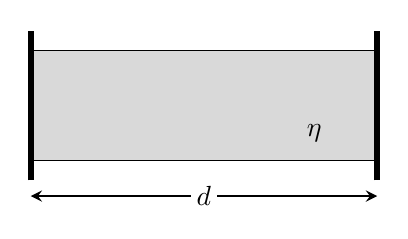
\begin{tikzpicture}[>=stealth, thick, scale=1.0]
  % Laser medium (shaded)
  \fill[black!15] (0, -0.7) rectangle (4.4, 0.7);
  \draw[thin] (0, -0.7) -- (4.4, -0.7) (0, 0.7) -- (4.4, 0.7);

  % Mirrors at x=0 and x=4.4
  \draw[line width=2.2pt] (0, -0.95) -- (0, 0.95);
  \draw[line width=2.2pt] (4.4, -0.95) -- (4.4, 0.95);

  % Refractive index label
  \node at (3.6, -0.35) {$\eta$};

  % Distance d
  \draw[<->] (0, -1.15) -- (4.4, -1.15) node[midway, fill=white, inner sep=2pt] {$d$};
\end{tikzpicture}
\end{document}
